\documentclass[final]{beamer}
\usepackage[T1]{fontenc}
\usepackage{lmodern}
\usepackage[size=custom,width=120,height=72,scale=1.0]{beamerposter}
\usetheme{gemini}
\usecolortheme{gemini}
\usepackage{graphicx}
\usepackage{booktabs}
\usepackage{tikz}
\usepackage{pgfplots}
\usepackage{csquotes}
\usepackage[
backend=biber,
style=numeric,
citestyle=numeric
]{biblatex}
\addbibresource{biblio.bib}

\usepackage[font=small,labelfont=bf]{caption} 

\newcommand{\compresslist}{
  \setlength{\itemsep}{1pt}
  \setlength{\parskip}{0pt}
  \setlength{\parsep}{0pt}}

\newcommand{\bfSigma}{\mbox{\boldmath$\Sigma$}}
\newcommand{\bfLambda}{\mbox{\boldmath$\Lambda$}}
\DeclareMathOperator*{\argmax}{\arg\!\max}
% ====================
% Lengths
% ====================

% If you have N columns, choose \sepwidth and \colwidth such that
% (N+1)*\sepwidth + N*\colwidth = \paperwidth
\newlength{\sepwidth}
\newlength{\colwidth}
\setlength{\sepwidth}{0.025\paperwidth}
\setlength{\colwidth}{0.3\paperwidth}
\newcommand{\separatorcolumn}{\begin{column}{\sepwidth}\end{column}}

% ====================
% Title
% ====================
\title{Text Sequence Generation and Classification: \textit{of the imitation of
Shakespeare}}
\author{Jimmy Leroux, Nicolas Laliberté, Frédéric Boileau}

\institute[]{Départment d'Informatique et de Recherche Opérationnelle -
Université de Montréal}

% ====================
% Body
% ====================

\begin{document}
\begin{frame}[t]
\begin{columns}[t]
\separatorcolumn

\begin{column}{\colwidth}

\begin{block}{Introduction}
\begin{itemize}
\item Hidden Markov Models used to be the go-to probabilistic tool to reason
    about sequential data; the Markov assumption however proves to often be
    unreasonably strong. Adding links to form higher order chains is not a
    scalable solution as the computationnal complexity grows exponentially in
    the order of the chain.

\item Recurrent Neural Networks (RNN) constitute a family of neural network
architectures specialized to process sequential data which can forfeit
Markovian assumptions while remaining tractable.

\item RNNs can track longer range dependencies while
    staying tractable by leveraging the simple idea of sharing parameters
    across the model \cite{deeplearning}. Concretely this means adding loops to
    the hidden units of the neural network.

\item RNNs have been successfully used in diverse domains for
  generating sequences such as music and text \cite{gravesGenerating}. 

\item Despite the aforementionned features, naive RNNs suffer from the fact 
that the influence of some input to the hidden layer either decays or blows up
exponentially in time, a phenomenon reffered to in the literature as the
\textit{vanishing gradient problem}.
\end{itemize}
The cost of abandonning probabilistic models such as the HMM in favor of neural
networks is the loss of a fully probabilistic interpretation. There has
recently been an increased interest into finding reasonable probabilistic
interpretaions to RNNs, see for example \cite{finnish}. On the other hand the
very existence of some monolithic notion of ``interpretability'' has been
recently questionned, see \cite{mythos} for a philosophically inclined take
on the question.
\end{block}

\begin{block}{RNN and the Vanishing Gradient} 
\begin{center}
    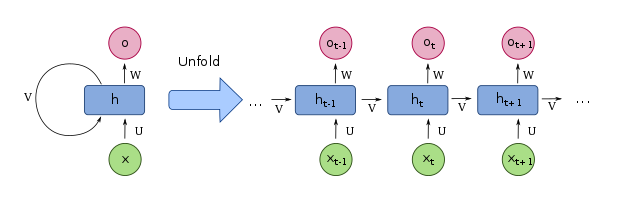
\includegraphics[width = 0.9\linewidth]{RNN.png}
\end{center}
\begin{equation*}
    h_t = \sigma(U x_t + V h_{(t-1)} + b_h)\text{,}
    \qquad o_t = \text{softmax}(W h_t + b_o)
\end{equation*}
\small{Where $ U$, $V$ and $W$ are weights matrix and the vectors $b$ are bias
parameters.}\\

\normalsize
Consider the gradient of $o_{t + \delta}$ with respect to $h_t$.\\
Applying the chain rule according to the graph above we get:

\begin{equation*}
  \nabla_{h_t} o_{t + \delta} = \left( \prod_{k = t+1}^{t+\delta} V^T
  \text{diag}(1 - h^2_k) \right)\nabla_{h_{t + \delta}}o_{t + \delta}.
\end{equation*}

Thus, as $\delta$ grows, the gradient grows exponentially with $V$. If $V$ is
small or large then the gradient will either vanish or explode. A myriad
of solutions exist such as regularization through weight noise, the Long Short
Term Memory architecture tries to tackle this issue on a higher level than
regularization.
\end{block}
\end{column}
\separatorcolumn

\begin{column}{\colwidth}

\begin{block}{LSTM Architecture}
To go from a RNN to a LSTM we replace hidden units with components known as
\textit{memory cells}. Our presentation and notation follows \cite{revieww}.
\begin{center}
    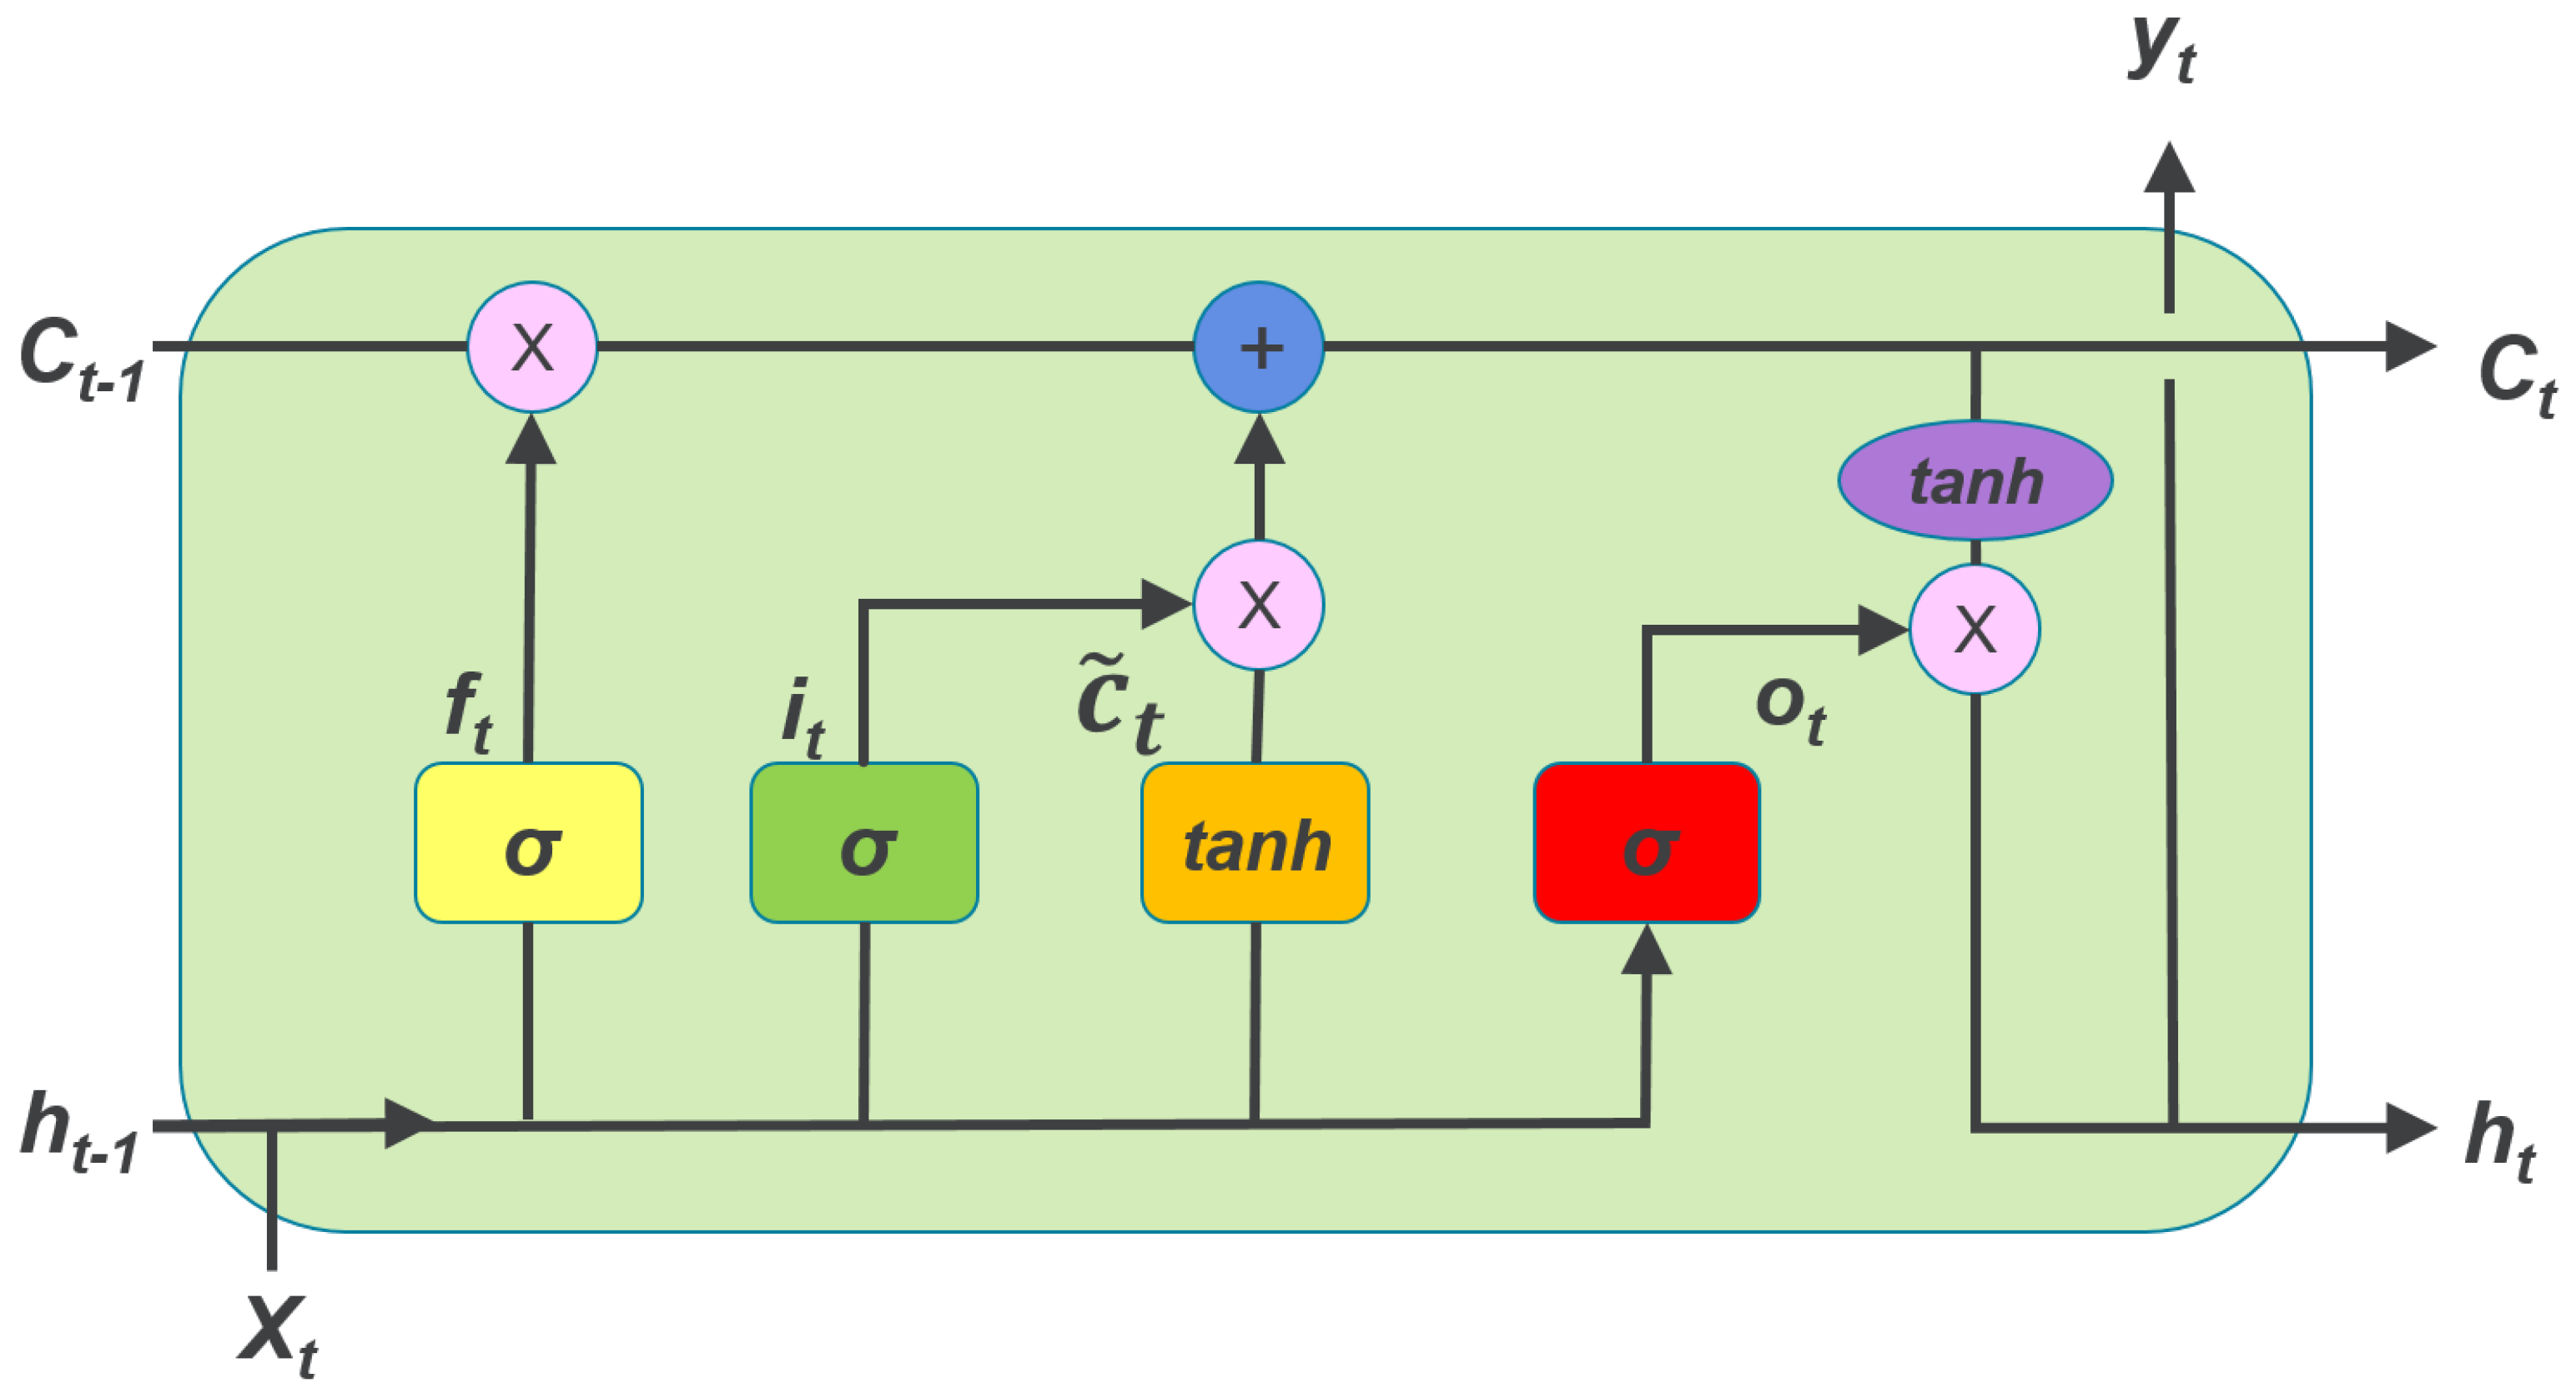
\includegraphics[width = 0.7\linewidth]{lstm.png}
\end{center}

Intuitively, RNNs have \textit{long-term memory} in the form of matrix weights,
they change during the training; encoding through training some general
knowledge about the data. They also have \textit{short-term memory} in the form
of activation passing from each node to successive ones. The memory cell
introduced in the LSTM model formalizes those notions and provides a framework
to control their impact on the internal representation of the network.
\begin{center}
    \begin{itemize}
    \item $f_t, i_t, o_t$: Respectively forget, input and output gates.
        \begin{itemize}
            \normalsize
            \item Sigmoidal units activated through  $x_t$ (current input) and
                $h_{t-1}$ (past hidden unit output) \item $f_t$ controls the
                recursive flow
            \item $i_t$ and $o_t$ control the input and output flow
                respectively
            \item $h_t = o_t \odot \tanh(c_t)$ where $\odot$ denotes element
                wise multiplication.
        \end{itemize}
    \item $c_t = \mathbf{f_t \odot c_{t-1}} + i_t \odot \tilde{c}_t$: The cell
    which has a self-connected edge with a fixed unit weight, thereby delegating
    control of recursion to the gate \end{itemize}
\end{center}

\end{block}

\begin{block}{Sequence Generation and Implementation Details}
    \begin{itemize}
        \item 4 text sequences (referred to as datasets later on) were used for
            training: excerpts from Shakespeare' plays, books of the Harry
            Potter and Lord of the Ring series and a list of popular quotes.
            All in English and ASCII encoded. Punctuation and structure was
            left unprocessed.
        \item Each dataset was split in sequences of 50 tokens (i.e. ``words'') and a
            dictionnary was built from the complete input ($\approx 60k$ unique tokens),
            defining the input space for the networks.
        \item Vector encoding of this space was used through an embedding layer 
            mapping the words to a real vector space of dimension 256. Available
            embeddings such as \textit{word2vec} and \textit{glove} were 
            initally used but proved to be more cumbersome than our own 
            trained version.
        \item 5 LSTM networks were trained with the above, 4
            \textit{generators} and a \textit{classifier}. Training
            was achieved at ``word'' level (strings tokenized by whitespace).
            Character level is envisionned for the rest of the project as it is
            more flexible and can \textit{learn new words and structural
            information} \cite{gravesGenerating} for the generators)
    \end{itemize}
To generate the sequences the trained models were initialized with a random word
drawn from the dictionary and the most likely next word was fed back in the network
until the desired sequence length was reached. 1000 sequences (250 per model) were
generated. The classifier was then used to automatically estimate which
dataset (or model, equivalently) was used for its generation, thereby giving us
some ``metric'' of the quality of the data; expecting data generated from the
Shakespeare trained model to consistenly differ from the data ``generated by
Harry Potter''.
\end{block}
\end{column}

\separatorcolumn

\begin{column}{\colwidth}

\begin{block}{Results}
 \begin{center}
	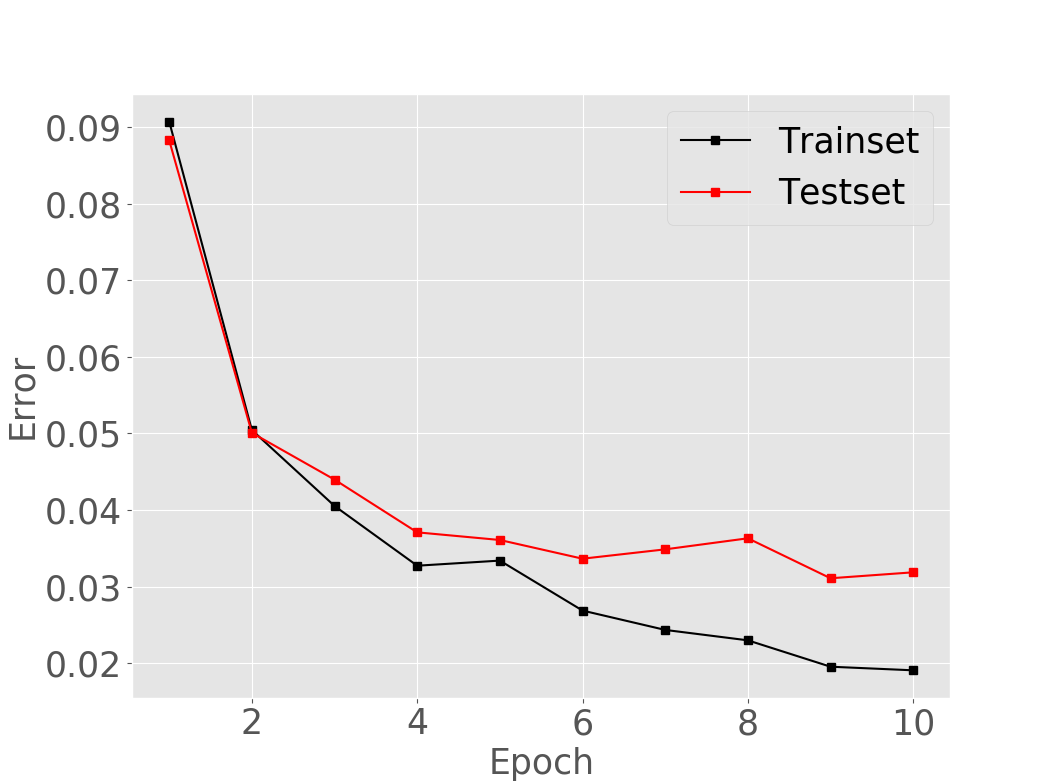
\includegraphics[width=.7\linewidth]{classerror}
	\captionof{figure}{Classification error on train/test set.}
\end{center}

Training trough minimization of the cross-entropy loss, which is equivalent to
\textit{perplexity}; the standard metric for language
modeling \cite{gravesGenerating}.
\begin{figure}[htbp!]
\begin{tabular}{|l|l|c|}
\hline
Dataset & BPC & Perplexity \\
\hline
Harry Potter & 1.00 & 33 \\
LOTR & 1.02 & 35 \\
Random quotes & 1.10 & 45 \\
Shakespeare & 0.94 & 26\\
\hline
\end{tabular}
\end{figure}

Examples of generated quotes:
\begin{itemize}\compresslist
    \item `` well , we ' ll do it with a wand , '' said hermione . `` really ?
      '' said harry , looking at each other .
    \item  what looked about this
      way , the black citadel , was far from the
          darkness , the ring was heard , but the sea big was big , and a great
          ring was in his battle .
    \item failure is a beginning of love and a family which comes from god .
    \item  '' that now my mind shall screens his music , '' '' and i to give
      thee my vulgar heaven , '' '' i am your brother .
\end{itemize}
\end{block}
\begin{block}{References}
\printbibliography
\end{block}
\end{column}
\separatorcolumn
\end{columns}
\end{frame}

\end{document}
